\documentclass{article}
\usepackage{tikz}
\usepackage[margin=1in]{geometry}
\usetikzlibrary{positioning}
\usetikzlibrary{shapes, arrows}
\begin{document}


\centerline{\sc \large Operating Systems Writeup}
\vspace{.5pc}

\begin{flushleft}
\textbf{Name:} Joshua Abraham
\vspace{.5pc}

\textbf{Date:} 2 November 2017
\vspace{.5pc}

\textbf{Current Module:} Operating Systems
\vspace{.5pc}

\textbf{Project Name:} "Relay"
\vspace{.5pc}

\textbf{Project Goals:}
\vspace{.5pc}
\end{flushleft}

The relay project aims to create two programs that communicate via Interprocess 
Communication.  This IPC will be one-way, from a "\textbf{dispatcher}" program 
that takes input from standard input to a "\textbf {listener}" program that 
prints text sent to the first program.
\vspace{.5pc}

\begin{flushleft}
\textbf{Considerations:}
\vspace{.5pc}
\end{flushleft}

\begin{itemize}
	\item[$\bullet$] \textbf{Dispatcher} must take text from stdin and exit when
	it receives an EOF.
	\item[$\bullet$] \textbf{Listener} should exit if the listener is closed or
	not running.
	\item[$\bullet$] Multiple \textbf{listeners} should be able to run 
	simultaneously from different users/directories.
\end{itemize}
\vspace{.5pc}

\begin{flushleft}
\textbf{Initial Design:}
\vspace{.5pc}
\end{flushleft}

The project is composed of the following files:
\begin{itemize}
	\item [$\cdot$] \textit{Makefile}: The main makefile for the project.
\end{itemize}
\vspace{2mm}

\begin{flushleft}
\textbf{Data Flow:}
\vspace{.5pc}
\end{flushleft}

The data flow from \textbf{dispatcher} to \textbf{listener} is as follows:

\begin{center}
\begin{equation}
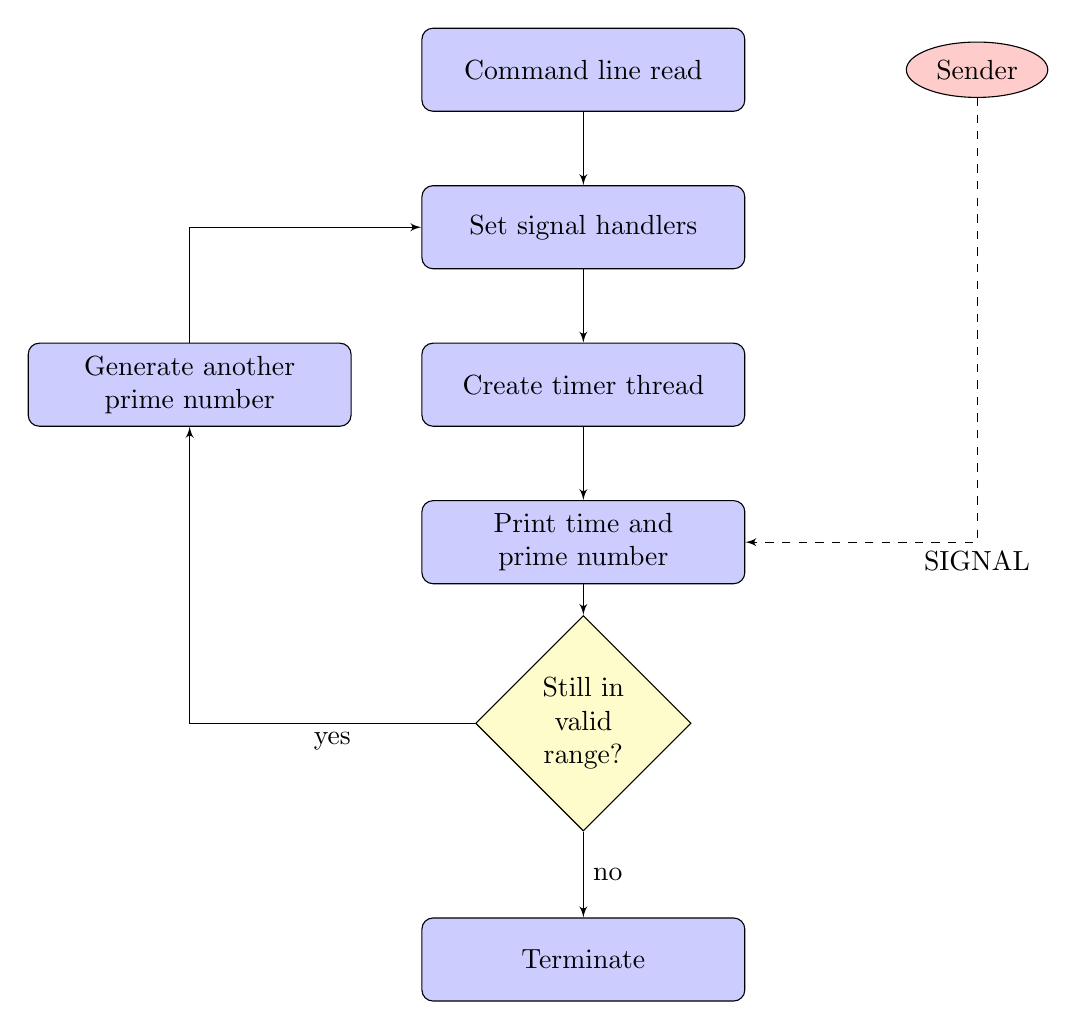
\begin{tikzpicture}[node distance = 2cm, auto]
    \tikzstyle{decision} = [diamond, draw, fill=yellow!20, 
    text width=4.5em, text badly centered, node distance=2.3cm, inner sep=0pt]
    \tikzstyle{block} = [rectangle, draw, fill=blue!20, 
    text width=11em, text centered, rounded corners, minimum height=3em]
    \tikzstyle{line} = [draw, -latex']
    \tikzstyle{cloud} = [draw, ellipse,fill=red!20, node distance=3cm,
    minimum height=2em]
    \node [block] (commands) {Command line read};
    \node [cloud, right of=commands, node distance=5cm] (sender) {Sender};
    \node [block, below of=commands] (sethandlers) {Set signal handlers};
    \node [block, below of=sethandlers] (evaluate) {Create timer thread};
    \node [block, below of=evaluate] (request) {Print time and prime number};
    \node [decision, below of=request] (keepmining) {Still in valid range?};
    \node [block, left of=evaluate, node distance=5cm] (anotherpath)
    {Generate another prime number};
    \node [block, below of=keepmining, node distance=3cm] (return) {Terminate};
    \path [line] (commands) -- (sethandlers);
    \path [line] (sethandlers) -- (evaluate);
    \path [line] (evaluate) -- (request);
    \path [line] (request) -- (keepmining);
    \path [line,dashed] (sender) |- node [midway, below] {SIGNAL} (request);
    \path [line] (keepmining) -| node [near start] {yes} (anotherpath);
    \path [line] (anotherpath) |- (sethandlers);
    \path [line] (keepmining) -- node {no}(return);
\end{tikzpicture}
\end{equation}
\end{center}

The basic flow of the signaler program is shown in figure 1.
The signaler gets its command line arguments and sets the appropriate flags 
and values.  It enters its main loop and sets its signal handlers.  Signaler
spawns a timer thread to pause its execution for .8 seconds.  It then prints 
the timestamp.  Lastly, signaler generates the next prime number in the 
sequence to be printed.  We do so with Fermat's little theorem, seen below:
We perform 4 rounds of the Fermat Primality Test.  This is a very fast and 
performant calculation. While this might be overkill for relatively small 
integers, this method will pay off when calculating extremely large primes.
\vspace{.5pc}

\begin{flushleft}
\textbf{Communications Protocol:}
\vspace{.5pc}
\end{flushleft}

The signaler and sender communicated via signals. We specifically use the 
SIGHUP, SIGUSR1, SIGUSR2, and SIGKILL. 
\vspace{.5pc}

\begin{flushleft}
\textbf{Potential Pitfalls:}
\vspace{.5pc}
\end{flushleft}

\begin{itemize}
	\item[$\bullet$] Prime generation taking too much time.
	\item[$\bullet$] Incorrectly handling signals.
	\item[$\bullet$] Pausing execution without sleep.
\end{itemize}
\vspace{.5pc}

\begin{flushleft}
\textbf{Test Plan:}
\vspace{.5pc}
\end{flushleft}

\textit{User Tests:}
\begin{itemize}
	\item[$\cdot$] Ran signaler and sender simultaneously.
	\item[$\cdot$] Ran signaler and sent signals with bash kill command. 
\end{itemize}

\textit{Test Cases:}
\begin{itemize}
	\item[$\cdot$] Unit tests for the prime number generation and Fermat's
	Little Theorem.
	\end{itemize}
\vspace{.5pc}

\begin{flushleft}
\textbf{Conclusion:}
\vspace{.5pc}
\end{flushleft}

The signaler project has been challenging and a learning experience. I learned 
about signals and threads while working on this project. Pausing execution 
without sleep was a fun challenge to solve. While writing the signaler, I
ran into bugs that were difficult to debug and required me to use GDB 
extensively. One example was resetting the signal handler every time a signal
was received. If I had more time to work on the project I would improve it
by implementing a more robust prime number generator such as Miller-Rabin.
Overall, it was a success and I am satisfied with what I wrote. 
\end{document}